\documentclass[]{article}

\usepackage{graphicx}
\usepackage{minted}
\usepackage[svgnames]{xcolor}
\usepackage[colorlinks=true, linkcolor=Maroon, urlcolor=Maroon]{hyperref}

% Title Page
\title{Project Report - Securing Information Exchange with Blockchain}
\author{Harsh Kedia}


\begin{document}
	\begin{titlepage}
    \begin{center}
        \vspace*{1cm}
 
        \Huge
        \textbf{Securing Information Exchange with Blockchain}
 
        \vspace{0.5cm}
        \LARGE
        Project Report
 		
 		\vfill
        \vspace{0.5cm}
 
        {\normalsize by}\\
        {\Large Harsh Kedia}
 
        \vfill
        \vspace{0.5cm}
        
        {\Large Supervisor: Thomas Hepp}\\
        {\Large Examiner: Prof. Dr. Bela Gipp}
 		
 		\vfill
 		\vspace{0.5cm}
 		
        \Large
        Department of Computer and Information Science\\
        Information Science Group\\
        University Of Konstanz\\
        \today
 
    \end{center}
\end{titlepage}
	
	\begin{abstract}
		Existing applications for sharing files are central solutions and therefore suffer from the single point of failure risk. Moreover, using central services for securing data means that we have to trust a 3rd party with our data thus exposing it to manipulation risks. Hence, a decentralized application was required to overcome the problems posed by a central application. With the recent developments in Blockchain technology and P2P storage, it is possible to securely store and share data without using any central server.
		
		This report outlines my master's project which is about securing information exchange using Blockchains. I describe here the workings of my application \textit{dShare} built using P2P technologies enabling a secure way of storing and sharing data between two individuals or entities.
		
		For storing files, I used the InterPlanetary File System (IPFS), which is a P2P file storage protocol. Before uploading to the IPFS network, files are encrypted using AES-GCM encryption mechanism. Sharing of keys is facilitated using smart contracts built on Ethereum; thus files can be shared by anyone having an Ethereum address. Finally, for immutable timestamping, OriginStamp is used, which submits a file's hash to the Bitcoin blockchain.
		
		I implemented the front-end using React.js, a JavaScript framework. Solidity was used to write smart contracts and deployed on the Ethereum test network (Rinkeby). Next.js was used for server-side rendering (SSR), and Firebase was used as a database for storing public Ethereum key of the users. The latest version of the application is deployed on Heroku at \href{https://file-share-dapp.herokuapp.com/}{https://file-share-dapp.herokuapp.com/}.
	\end{abstract}
	
	\newpage
	\section{Project Motivation}
		Today's supply chain spans multiple geographies, but the documents involved in the industry such as delivery certificates are still in physical form. This paperwork prevents manipulations but leads to various delays across the whole chain, thus affecting everyone involved\footnote{\url{https://www-01.ibm.com/common/ssi/cgi-bin/ssialias?htmlfid=XI912347USEN}}.
		
		The above problem can be solved by digitizing all documents, time-stamping them using a trusted Time stamping authority (TSA) and upload them to a cloud service. However, the tools used to accomplish this solution are central services, and, therefore, suffers from data manipulations by a 3rd party.
		
		We, therefore, need a solution that is peer-to-peer (P2P) and decentralized. Blockchain offers a means of decentralized time stamping and enables peer-to-peer storage systems that are resistant to manipulations by any 3rd party.
		
		This project describes the working of an application build using decentralized technologies such as Bitcoin\cite{nakamoto2008bitcoin}, Ethereum\cite{buterin2014next} and IPFS\cite{benet2014ipfs} such that it is capable of immutable timestamping and secure file sharing in a P2P manner.
		
	\newpage
	\section{Related Work}
		Trusted timestamping is a way of verifying that specific information existed at a given point in time. Blockchains enables anchoring of data utilizing cryptocurrency transactions where each transaction gets an immutable timestamp. 
		
		Blockchains also enables the creation of smart contracts. Smart contracts are computer codes stored on the blockchain encoding the terms of a contract. It helps in negotiating and enforcing an agreement without any third parties involved.
		
		Finally, P2P protocols such as BitTorrent\cite{levin2008bittorrent}, Distributed Hash Tables (DHT), and Git enables us to secure information distributes across multiple computers.
		
		Below sections explore the state-of-the-art in decentralized timestamping and decentralized storage.
		
		
		\subsection{Proof of Existence}
			Proof of Existence\footnote{\url{https://poex.io/}} is a web-based service that implements the concept of immutable timestamping using the Bitcoin blockchain. It notarizes data in the blockchain by submitting the hash of the data in a Bitcoin transaction. Currently, the service required 0.00025BTC\footnote{\url{https://poex.io/prove}} for every certification which makes it expensive to timestamp large volumes of data.
			
		\subsection{OriginStamp}
			OriginStamp\cite{gipp2015decentralized}\footnote{\url{https://originstamp.org/}} extends the concept of Proof of Existence by providing a scalable protocol which overcomes the transaction limitations of the Bitcoin blockchain.
			
			When a user submits a file, the hash of the data is recorded. Instead of creating a Bitcoin transaction for each submitted hash, it combines all the hashes submitted over a time period and generates an aggregated hash. After some additional hashing and encoding operations, a Bitcoin address is created, to which the smallest possible transactional amount of Bitcoins is transferred. Performing this transaction embeds the hash and the timestamp permanently to the Bitcoin blockchain.
			
		\subsection{Chainpoint}
			Chainpoint\footnote{\url{https://chainpoint.org/}} works similarly to OriginStamp. The service runs on the Tierion\footnote{\url{https://tierion.com/}} Network, providing a scalable protocol for anchoring data in the blockchain and generating blockchain receipts. These receipts are called chainpoint proofs which defines a path of operations that cryptographically links the data to one or more blockchains.
			
		\subsection{Sia}
			Sia\cite{vorick2014sia} is a decentralized cloud storage system that allows its users to rent storage among peers utilizing storage contracts which are cryptographically secured by saving on a blockchain. This makes the storage contracts tamper-proof and publicly auditable.
			
			To ensure that the storage provider holds a client’s data at a given time, they constantly need to submit storage proofs. The network consensus allows automatic verification of storage proofs and enforcement of storage contracts. The availability of data is ensured using redundancy techniques such as erasure codes.
			
			Sia uses a variant of Bitcoin blockchain for storing the contracts, and the user must use Siacoin, an ERC-20\footnote{\url{https://theethereum.wiki/w/index.php/ERC20_Token_Standard}} token in order to transact on the Sia network.
		
		\subsection{Storj}
			Storj\cite{wilkinson2014storj} works similarly to Sia. It is built on Kademlia\cite{maymounkov2002kademlia} DHT, connecting peers who can transact with each other. A transaction can involve negotiation of storage contract, transfer of data, verifying remote data, download data or payments to other nodes. Each peer is capable of doing transactions independently without any human involvement.
			
			Storj uses the Ethereum blockchain for managing its storage contracts. They are stored as versioned data structure describing the relationship between a client and a storage provider. Users must use Storjcoin, an ERC-20 token to perform transactions on the Storj network. 
		
		\subsection{InterPlanetary File System (IPFS)}
			Unlike Sia and Storj, IPFS\cite{benet2014ipfs} is a P2P file transfer protocol which connects all peers in the network by a shared file system. It achieves this by combining previous peer-to-peer systems such as DHT, BitTorrent, and Git. The data in the IPFS network are modeled as a Merkle\cite{merkle1980protocols} DAG thus providing a throughput storage system with content-addressed hyperlinks.
			
			To transact on the IPFS network, a user does not need any tokens.
	
	\newpage
	\section{Approach}
		This section compares the current state-of-the-art in decentralized timestamping and decentralized storage and provides an approach for building a secure information exchange overcoming the limitations of the existing systems.
		
		\begin{figure}[h]
			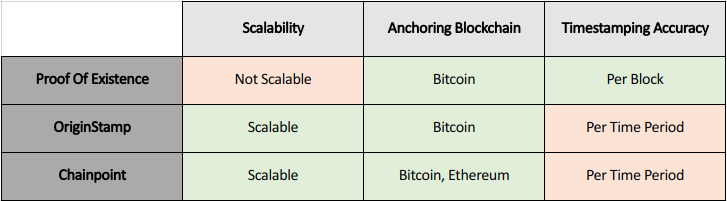
\includegraphics[width=\linewidth]{comparison-timestamping.png}
			\caption{Comparing Decentralized Timestamping}
			\label{fig:comparison-timestamping}
		\end{figure}
	
		Comparing the decentralized timestamping solutions, Proof of Existence creates a Bitcoin transaction for each hash submitted by the user. Moreover, each certification costs 0.00025 BTC. These limitations make it impractical and expensive for timestamping a large volume of data. Both OriginStamp and Chainpoint, instead of creating a transaction for each submitted hash, concatenates the submitted hashes over a period and creates a single transaction with the aggregated hash. Thus they overcome the limitations of Proof of Existence and provide a scalable protocol which can handle large volumes of data.
	
		\begin{figure}[h]
			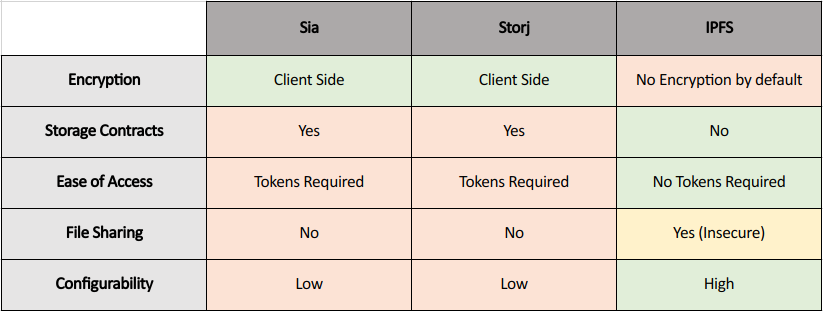
\includegraphics[width=\linewidth]{comparison-storage.png}
			\caption{Comparing Decentralized Storage}
			\label{fig:comparison-storage}
		\end{figure}
	
		Comparing the decentralized storage systems, both Sia and Storj provide encrypted data storage; however current implementations do not allow for file sharing. Moreover, both require platform specific crypto tokens to access the network. IPFS, on the other hand, does not encrypt files by default. Files on the IPFS network are accessed by their hashes; thus anyone who knows the file’s hash can access the file. There are no storage contracts involved for storing files on the network. IPFS network does not require any crypto token for the users to access the network.
		
		Looking at the limitations of the existing solutions, we propose a solution for secure information exchange with blockchains using smart contracts, permanent timestamping and decentralized storage.
		
		For timestamping both OriginStamp and Chainpoint can be used as they can handle large volumes of data and provide a rich set of APIs for integrating decentralized timestamping in any application. For decentralized storage, we want to use IPFS as it is a general-purpose file storage protocol and does not require any crypto tokens for access to its network and for exchanging document encryption keys, we want to use the Ethereum smart contracts.
	
	\newpage
	\section{Implementation}
		This section describes the workings of the different components of the \textit{dShare} application.
		
		\subsection{Smart Contract}
		The smart contract serves as the bridge between the front-end of the application and the Ethereum Blockchain. Data is read from and written to the blockchain with the help of function calls in the contract. Each function call which modifies some data requires a small fee in the form of gas\footnote{\url{https://ethereum.stackexchange.com/questions/3/what-is-meant-by-the-term-gas}} which defines the cost for a function execution in Ether. Reading from the blockchain does not require any fees.
		
		\textit{dShare} makes use of two contracts, \textit{FileFactory}, which acts as the factory contract for creation of new files and \textit{File}, which represents an individual file.
		
		\subsubsection{FileFactory Contract}
		\textit{FileFactory} is the contract which is deployed on the Rinkeby test network. It has several \textit{mappings} which stores the list of file contracts uploaded by a user. Below is a list of variables used to store relevant data regarding files.
		
\begin{minted}{js}
/// @notice Stores the list of files deployed by an address
mapping(address => address[]) uploadedFiles;

/// @notice Stores the list of files shared by an address
mapping(address => address[]) sharedFiles;

/// @notice Stores the list of files shared with an address
mapping(address => address[]) recipientFiles;

/// @notice Stores the list of files archived by all users
address[] archivedFiles;

/// @notice List of Uploaders
mapping(address => bool) uploaders;

/// @notice List of Recipients
mapping(address => bool) recipients;
\end{minted}

		Whenever a user uploads a file, a function call is made to the \textit{FileFactory} contract, which in turn deploys the \textit{File} contract and updates the \textit{mappings} for \texttt{uploadedFiles} and \texttt{uploaders}.
		
\begin{minted}{js}
/// @notice Deploys a file contract to the blockchain
/// @dev Deploys a new contract which stores file details
/// @param _d Hash function digest
/// @param _h Hash function code
/// @param _s Size of _digest in bytes
/// @param _f sha3 hash of the uploaded file
function createFile(bytes32 _d, uint8 _h, uint8 _s, bytes32 _f) public {
  address newFile = new File(_d, _h, _s, _f, this, msg.sender);
  uploadedFiles[msg.sender].push(newFile);
  uploaders[msg.sender] = true;
}
\end{minted}

		\subsubsection{File Contract}
		\textit{File} contract is deployed to the blockchain whenever a file is successfully uploaded to the IPFS network using \textit{dShare}. Upon deployed, the \texttt{constructor} function is called. It takes the values passed by the \textit{FileFactory} contract and saves the details to it's \textit{File} contract.
		
\begin{minted}{js}
/// @notice Initializes the variables with values passed by the factory
/// @dev The constructor calles upon file deployment
/// @param _d Hash function digest
/// @param _h Hash function code
/// @param _s size of _digest in bytes
/// @param _fi sha3 hash of the file
/// @param _fa The address of the factory contract
/// @param _c The address of the uploader
constructor(bytes32 _d,uint8 _h,uint8 _s,bytes32 _fi,address _fa,address _c) public {
  fileIpfsHash = Multihash(_d, _h, _s);
  manager = _c;
  sha3hash = _fi;
  ff = FileFactory(_fa);
}
\end{minted}

		Below is a list of variables, a \textit{File} contract uses to store a file's details.
		
\begin{minted}{js}
/// @notice The address of the uploader
address public manager;

/// @notice sha3 hash of the file
bytes32 sha3hash;

struct Multihash {
  bytes32 digest;
  uint8 hashFunction;
  uint8 size;
}

/// @notice The address of the factory contract
FileFactory ff;

/// @notice The IPFS hash of the file
Multihash fileIpfsHash;

/// @notice List of recipients the file is shared with
address[] recipientsList;

/// @notice Stores the encrypted key's IPFS hash for each recipient
mapping(address => Multihash) keyLocation;
\end{minted}
		
		\newpage
		\subsection{File Upload}
		Figure ~\ref{fig:upload} visualizes the working of the application when a user uploads a file.
		
		\begin{figure}[h]
			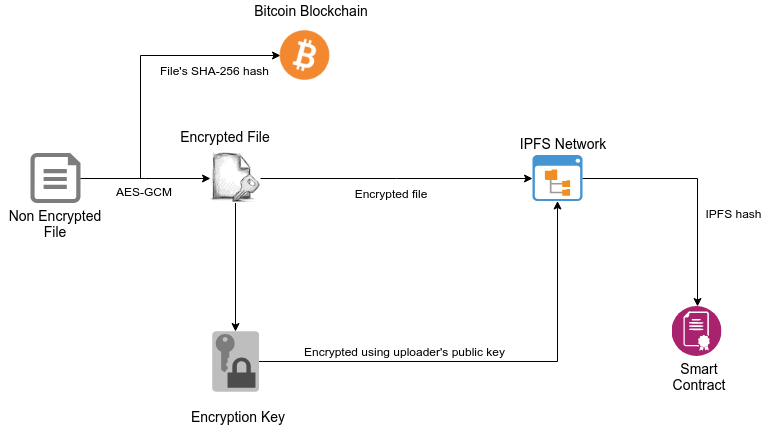
\includegraphics[width=\linewidth]{upload.png}
			\caption{Uploading a File using \textit{dShare}}
			\label{fig:upload}
		\end{figure}
		
		As soon as a user submits a file to be uploaded, it's SHA-256\footnote{\url{https://www.movable-type.co.uk/scripts/sha256.html}} hash is calculated and a timestamp is created by submitting the hash to the bitcoin blockchain using the OriginStamp API\footnote{\url{http://doc.originstamp.org/}}.
		
\begin{minted}{js}
// get the sha256 hash of file
const sha256hash = await sha256(this.state.buffer);

// create timestamp
try {
  await createTimeStamp(sha256hash, this.state.email);
} catch (error) {
  toast.error("Error in creating timestamp");
  return;
}
\end{minted}

		Next, the file is encrypted using the SubtleCrypto\footnote{\url{https://developer.mozilla.org/en-US/docs/Web/API/SubtleCrypto}} interface with 'AES-GCM'\footnote{\url{https://en.wikipedia.org/wiki/Galois/Counter_Mode}} as the encrypting algorithm. The encrypted data is then combined with the random salt to generate a \texttt{Uint8Array} buffer ready to be uploaded to the IPFS network.

\begin{minted}{js}
// encrypt the file
const { data, iv, key } = await encrypt(this.state.buffer);
const dataArray = new Uint8Array(data);

//combine the data and random value
const data_iv = new Uint8Array([...dataArray, ...iv]);
\end{minted}

		The key used to encrypt the file is converted to \texttt{JSON} and is encrypted using the uploader's Ethereum public key which is retrieved from the database.
		
\begin{minted}{js}
//encryption key in JSON
const keyData = await window.crypto.subtle.exportKey("jwk", key);

// getting the public key
const snapshot = await db
  .ref("/users/" + this.state.account.toLowerCase())
  .once("value");
const publicKey = snapshot.val() && snapshot.val().public_key;

//encrypt the document key with user's ethereum public key
const encryptedKey = await EthCrypto.encryptWithPublicKey(
  publicKey,
  Buffer.from(JSON.stringify(keyData))
);
\end{minted}

		This encrypted key and the encrypted data is then uploaded to the IPFS network.
		
\begin{minted}{js}
//Contruct the data to be uploaded to ipfs
const ipfsPayload = [
{
  path: `/tmp/${this.state.fileName}`,
  content: Buffer.from(data_iv)
},
{
  path: `/tmp/${this.state.account}`,
  content: Buffer.from(JSON.stringify(encryptedKey))
}
];

// uploading file to ipfs
await ipfs.files.add(ipfsPayload, (err, res) => {
  if (err) {
    console.error(err);
    return;
  }
  this.setState({ fileIpfsHash: res[2].hash }, () => {
    this.createFile(this.state.fileIpfsHash, sha256hash);
  });
});
\end{minted}

		Once the file is successfully uploaded, \texttt{createFile()} in the \texttt{FileFactory} contract is called which deploys a new \texttt{File} contract with all details regarding the file saved to the blockchain.
		
\begin{minted}{js}
createFile = async (fileIpfsHash, sha256hash) => {
  const { digest, hashFunction, size } = getBytes32FromMultiash(fileIpfsHash);

  try {
    await factory.methods
    .createFile(digest, hashFunction, size, "0x" + sha256hash)
    .send({
      from: this.state.account
    });
    Router.push("/files/");
  } catch (error) {
    toast.error(error.message);
  }
  this.setState({ loading: false });
};
\end{minted}
		
		\newpage
		\subsection{File Sharing}
		Sharing a file requires the recipient's Ethereum address and uploader's private key. Figure ~\ref{fig:share} visualizes the working of the application when a user shares a file with another user.
		
		\begin{figure}[h]
			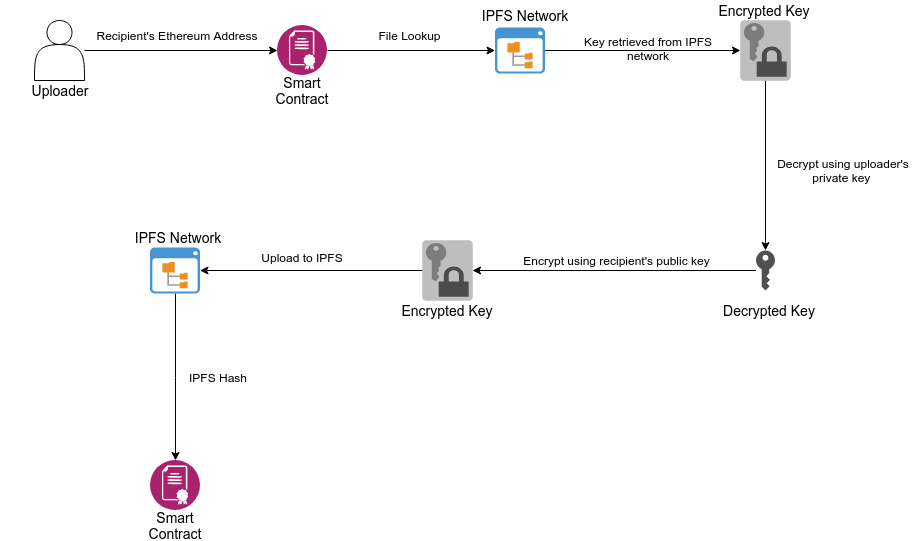
\includegraphics[width=\linewidth]{share.png}
			\caption{Sharing a File using \textit{dShare}}
			\label{fig:share}
		\end{figure}
	
		Firstly, the file's IPFS location is retrieved from the \texttt{File} contract. From this location, the encrypted key is download and decrypted using uploader's private key.
		
\begin{minted}{js}
// get File's IPFS hash from Contract
const returnedHash = await fileInstance.methods.getFileDetail().call({
  from: accounts[0]
});

// Retrive the encrypted key
await ipfs.files.cat(
  `${this.state.fileIpfsHash}/${accounts[0]}`,
  (err, file) => {
    this.setState({ fileEncryptedkey: JSON.parse(file.toString("utf8")) });
  }
);

// Decrypt the file key using user's private key
let decryptedKey;
try {
  decryptedKey = await EthCrypto.decryptWithPrivateKey(
    this.state.userPrivateKey,
    this.state.fileEncryptedkey
  );
} catch (error) {
    toast.error("Invalid Private Key");
    this.setState({ loading: false });
    return;
  }
\end{minted}

		Once decrypted, the key is again encrypted using a recipient's public key. The new encrypted key is again uploaded to the IPFS network.
		
\begin{minted}{js}
// Encrypt the file key using recipient's public key
const keyForSharing = await EthCrypto.encryptWithPublicKey(
  recipientPublicKey,
  Buffer.from(JSON.stringify(JSON.parse(decryptedKey)))
);

// Contruct the ipfs payload
const ipfsPayload = [
{
  path: `${this.state.recipient}`,
  content: Buffer.from(JSON.stringify(keyForSharing))
}
];

// uploading to ipfs
await ipfs.files.add(ipfsPayload, (err, res) => {
  if (err) {
    return;
  }
  this.setState({ keyIpfsHash: res[0].hash }, () => {
    this.shareFile(this.state.keyIpfsHash);
  });
});
\end{minted}

		Finally, the IPFS location is the key is saved into the \texttt{File} contract by calling \texttt{shareFile()}.
		
\begin{minted}{js}
try {
  await fileInstance.methods
    .shareFile(this.state.recipient, digest, hashFunction, size)
    .send({ from: this.state.account });

    Router.push("/files/");
  } catch (error) {
    toast.error(error.message);
  }
\end{minted}
		
		\newpage
		\subsection{File Download}
		Downloading a file requires the user's Ethereum private key. Depending on whether the file is uploaded or shared one, corresponding function from the \texttt{File} contract is called to retrieve the file's details.
		
\begin{minted}{js}
/** Retrieve the File Name */
await ipfs.files.get(this.state.fileIpfsPath, (err, files) => {
  if (err) {
    throw err;
  }
  this.setState({
  fileName: files[2].path.split("/").pop(),
  fileContent: files[2].content
  });
});

/** Retrive the encrypted key */
await ipfs.files.cat(this.state.keyIpfsPath, (err, file) => {
  if (err) {
    throw err;
  }
  this.setState({ encryptedKey: JSON.parse(file.toString("utf8")) });
});
\end{minted}
		
		The key is then decrypted using user's private key and is converted to a valid JSON web key (jwk)\footnote{\url{https://tools.ietf.org/html/rfc7517}} format.
		
\begin{minted}{js}
/** Decrypt the key using user's private key */
let decryptedKey;
try {
  decryptedKey = await EthCrypto.decryptWithPrivateKey(
    this.state.userPrivateKey,
    this.state.encryptedKey
  );
} catch (error) {
  toast.error("Invalid Private Key");
  this.setState({ loading: false });
  return;
}

/** Convert key into valid jwk format */
const key = await window.crypto.subtle.importKey(
  "jwk",
  JSON.parse(decryptedKey),
  "AES-GCM",
  true,
  ["encrypt", "decrypt"]
);
\end{minted}

		The encrypted file data is then converted to a file buffer, and the original file content and the random salt used for encrypting the file is retrieved.
		
\begin{minted}{js}
// Retrieve the original file Content
const fileBuffer = fileContent.slice(0, fileContent.length - 12);

// Retrive the original random nonce used for encrypting
const iv = fileContent.slice(fileContent.length - 12);
\end{minted}

		Finally, the file is decrypted and saved to the user's local storage.
		
\begin{minted}{js}
// Decrypt the file
const decryptedFile = await decrypt(fileBuffer, key, iv);

// Contruct the file
const file = new File([decryptedFile], this.state.fileName);
FileSaver.saveAs(file);
\end{minted}

		To stop sharing a file, a function call can be made to the \texttt{File} contract with the recipient's address, which deletes the contract reference from the \texttt{recipientFiles} array.
		
\begin{minted}{js}
/// @dev Removes the file's address from sharedFiles and recipientFiles
/// @param _iO The index of file in sharedFiles
/// @param _iR The index of file in recipientFiles
/// @param _r The address of recipient
/// @param _f the Address of uploader
function stopS(uint _iO,uint _iR,address _r,address _f) public isUploader(_f) {
  removeByIndex(_iO, sharedFiles[_f]);
  removeByIndex(_iR, recipientFiles[_r]);
}
\end{minted}
		
		\newpage
		\subsection{File Archiving}
		Instead of deleting a \texttt{File} contract, \textit{dShare} provides a way to achieve files. This is also useful to keep track of archived files and restore them at a later date if required.
		
		When a file is archived, the \texttt{File} contract address is saved in an array which is later used for filtering the archived files from the UI.
		
		Restoring a file removes the \texttt{File} contract address from the archived files array.
		
\begin{minted}{js}
/// @dev Adds the archieved file address to archivedFiles array
/// @param _file The address of the deployed file to be archived
/// @param _from the address of the uploader
function archiveFile(address _file, address _from) public isUploader(_from){
  archivedFiles.push(_file);
}

/// @dev Deletes the specified entry from archiveFile array
/// @param _index The index of the file in archiveFile array
/// @param _from The address of the uploader
function restoreFile(uint _index, address _from) public isUploader(_from) {
  removeByIndex(_index, archivedFiles);
}

/// @dev Function to delete element from an array
/// @param _index The index of element to be removed
/// @param _array The array containing the element
function removeByIndex(uint _index, address[] storage _array) internal {
  _array[_index] = _array[_array.length - 1];
  delete _array[_array.length - 1];
  _array.length--;
}
\end{minted}
	
	\newpage
	\section{Results}
		Blockchain and P2P technologies enable us to build a file sharing system that is both secure and decentralized. This distributes trust across the system and eliminates the single point of failure risk as seen in central services.
		
		This report presents the workings of \textit{dShare}; a secure file sharing application built using decentralized technologies such as Bitcoin, Ethereum and IPFS.
	
	\newpage
	\section{Future Work}
		Blockchain technology is still in its infancy. Most of the technologies used in this project are in alpha stage and therefore has quite a few bugs. \textit{dShare's} sharing logic is built using Ethereum smart contracts which have scaling issues are quite expensive to use at the moment. Therefore, for future work, I want to explore other P2P technologies which can make the existing implementation of the application more scalable and inexpensive to use.
		
		Latest Blockchain and P2P protocols such as Blockstack\footnote{\url{https://blockstack.org/}} and uPort\footnote{\url{https://www.uport.me/}} for decentralized identity management, 3Box\footnote{\url{https://3box.io/}} for app-specific data store and OrbitDB\footnote{\url{https://github.com/orbitdb/orbit-db}} for P2P databases can enhance the functionalities of \textit{dShare} and make it more scalable and inexpensive.
	
	\newpage
	\bibliographystyle{acm}
	\bibliography{report}
\end{document}          
